%  !TeX  root  =  user_guide.tex

\chapter{Primeiros Passos}\label{label_getstarted}

% when the revision of a section has been finalized, 
% comment out the following line:
% \updatedisclaimer

Este capítulo dá uma rápida noção de como instalar o \qg, como executar uma primeira sessão
com visualização de imagens e vectores com dados 
de exemplo disponíveis na página internet do \qg.


\section{Instalação}\label{label_installation}
\index{Instalaçao}

Instalar o \qg é muito simples. Existem pacotes de instalação 
disponíveis para MS Windows e Mac OS X. Para muitas distribuições de GNU/Linux 
(rpm e deb) ou repositórios de software para adicionar ao gestor de instalaçao ?????
Receba as últimas informações sobre pacotes binários no 
Website do \qg em \url{http://qgis.osgeo.org/download/}.

\minisec{Instalaçao do Código Base}

Caso pretenda complilar o \qg do código, consulte o código e o 
gui da compilaçao disponível em \url{http://qgis.osgeo.org/documentation/}. 
As instruções de instalaçao são também disponibilizadas com o código fonte do \qg.

\minisec{Instalação em mídia externo}

QGIS permite definir um "--configpath option" que substitui a localização predefinida 
(exemplo ~/.qgis em Linux) para a configuração do utilizador e força o "QSettings" a usar 
este directório. Isto permite aos utilizadores por exemplo realizar uma instalaçao de QGIS numa 
unidade flash juntamente com todos os plugins e configurações. 

\section{Dados Exemplo}\label{label_sampledata}
\index{data!sample} 

O manual de utilizador contém exemplos baseados nos dados de exemplo do \qg. 

\win A instalaçao para Windows tem a opção de download dos dados de exemplo do \qg.
Caso a opção esteja assinalada, os dados serão transferidos para a pasta \filename{Meus Documentos}
numa pasta designada de \filename{GIS Database}. 
Pode usar o Windows Explorer para mover a pasta para outro local.
Caso não pretenda seleccionar esta opção, 
durante a instalaçao do \qg, poderá:
\begin{itemize}[label=--]
\item utilizar dados que disponha;
\item efectuar o download dos dados de exemplo do website \url{http://qgis.osgeo.org/download}; ou
\item desinstalar o \qg e reinstalar com a opção de dados de exemplo seleccionada, apenas no caso de 
a opção anterior não ser bem sucessida.
\end{itemize}

\nix \osx Para GNU/Linux and Mac OSX ainda não existem pacotes de instalação com dados
de exemplo como é o caso de rpm, deb ou dmg. Para utilizar os dados de exemplo deverá fazer o download 
do ficheiro \filename{\qg\_sample\_data} em ficheiro ZIP ou TAR  de
\url{http://download.osgeo.org/qgis/data/} depois descomprime para uma pasta no
sistema.O conjunto de dados Alaska inclui todos os dados SIG que são utilizados como
exemplo e capturas de ecrân do manual de utilizador, assim como alguma informação para o GRASS.
A projecção para os dados de exemplo do Alaska Alaska Albers Equal
Area com unidades em pés. O código EPSG é o 2964.

\begin{verbatim}
PROJCS["Albers Equal Area",
    GEOGCS["NAD27",
        DATUM["North_American_Datum_1927",
            SPHEROID["Clarke 1866",6378206.4,294.978698213898,
                AUTHORITY["EPSG","7008"]],
            TOWGS84[-3,142,183,0,0,0,0],
            AUTHORITY["EPSG","6267"]],
        PRIMEM["Greenwich",0,
            AUTHORITY["EPSG","8901"]],
        UNIT["degree",0.0174532925199433,
            AUTHORITY["EPSG","9108"]],
        AUTHORITY["EPSG","4267"]],
    PROJECTION["Albers_Conic_Equal_Area"],
    PARAMETER["standard_parallel_1",55],
    PARAMETER["standard_parallel_2",65],
    PARAMETER["latitude_of_center",50],
    PARAMETER["longitude_of_center",-154],
    PARAMETER["false_easting",0],
    PARAMETER["false_northing",0],
    UNIT["us_survey_feet",0.3048006096012192]]
\end{verbatim}

Caso pretenda utilizar o \qg como frontend gráfico do GRASS, poderá encontrar
uma variedade de dados (exemplo: Spearfish ou South Dakota) no site oficial do
GRASS GIS \\
\url{http://grass.osgeo.org/download/data.php}. 

\section{Sessão de Exemplo}\label{samplesession}

Após a instalaçao do \qg installed e com dados de exemplo disponíveis , podemos 
testar algumas funcionalidades do \qg. Poderemos visualizar 
um raster e um layer de vectores. Utilizamos o raster landcover 
layer \filename{\qg\_sample\_data/raster/landcover.img} e o layer de vectores lakes 
\filename{\qg\_sample\_data/gml/lakes.gml}.

\minisec{start \qg}

\begin{itemize}[label=--]
\item \nix{Execute o \qg escrevendo: \usertext{\qg} na linha de comando, ou
no caso de uma versão pré-complilada, usando o Menu das Aplicações.}
\item \win{Execute o \qg utilizando o Menu Iniciar ou o atalho no Ambiente de Trabalho, 
ou com duplo clique sobre um projecto \qg.}
\item \osx{Duplo clique no icon na pasta das aplicações.}
\end{itemize} 

\begin{figure}[ht]
   \centering 
   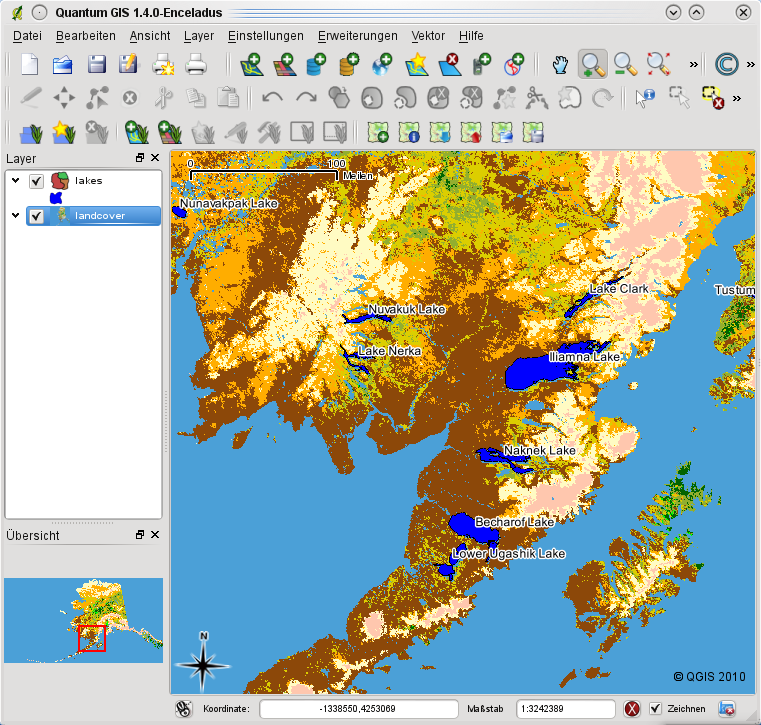
\includegraphics[clip=true, width=12cm]{simple_session}
   \caption{Uma sessão simples de \qg \nixcaption}\label{fig:simple_session}
\end{figure}

\minisec{Carregar um layer de raster e vector dos dados de exemplo}

{\setlength{\baselineskip}{1.3\baselineskip}
\begin{enumerate}[itemsep=2pt]
\item Click no botão \toolbtntwo{mActionAddRasterLayer}{Load Raster}.
\item Pesquise na pasta \filename{\qg\_sample\_data/raster/}, seleccione
o ficheiro da imagem ERDAS \filename{landcover.img} e clique em \button{Open}.
\item Se o ficheiro não surgir na lista, verifique se a Combobox dos tipos de ficheiro no
fundo da caixa de diálogoestá definido correctamente, neste caso "Erdas Imagine
Images (*.img, *.IMG)"
\item Clique no botão \toolbtntwo{mActionAddOgrLayer}{Load Vector}. 
\item \radiobuttonon{'File'} deverá estar seleccionado no separador "Source Type"
da caixa de dialogo \dialog{Add Vector Layer}. De seguida carregue emn \button{Browse} para seleccionar o
ficheiro (layer de vectores).
\item Navegue até à pasta \filename{\qg\_sample\_data/gml/}, seleccione "GML"
na combobox dos tipos de ficheiro, abra o ficheiro GML \filename{lakes.gml} 
e carregue no botão \button{Open}, depois na caixa de dialogo "Add Vector" carregue em \button{OK}.
\item Faça um zoom numa área à escolha com alguns lagos.
\item Faça duplo clique no layer \filename{lakes} na legenda do mapa, para abrir a 
caixa de dialogo \dialog{Layer Properties}.
\item Clique no separador \tab{Symbology} e seleccione o azul como cor de preenchimento (fill color).
\item Click no separador \tab{Labels} e active \checkbox{Display labels} 
para activar as labels. Escolha o campo NAMES como campo com a legenda.
\item Para melhorar a leitura da legenda, poderá colocar um buffer branco em torno da legenda,
clicando em ``Buffer'' na lista à esquerda, activando \checkbox{Buffer
labels?} e o valor de 3 para o buffer.
\item Carregue em \button{Apply}, e verifique no mapa o resultadoe finalmente 
carregue em  \button{OK}.
\end{enumerate} 
\par}
Como pode constatar é muito fácil visualizar rasters e layers vectoriais no 
\qg. Nas próximas secções iremos aprender mais acerca 
das funcionalidades disponíveis, recursos e configurações e como as usar.

\FloatBarrier
